\documentclass{report}
\usepackage[left=2cm,right=2cm,top=2cm,bottom=2cm,bindingoffset=0cm]{geometry}
\usepackage[utf8x]{inputenc}
\usepackage[english,russian]{babel}
\usepackage{amsfonts}
\usepackage{amsmath}
\usepackage{mathtools}

\usepackage{graphicx}
\graphicspath{{pictures/}}
\DeclareGraphicsExtensions{.pdf,.png,.jpg}

\begin{document}
\LARGE{ \textbf {Лекция №7}}\\
\Large{ \textbf {}}\\
Данный триггер реализованый в базисе ИЛИ-НЕ является триггером с прямыми входами.
Прямые входы означают, что активным уровнем управляющих сигналов является уровень логической единицы.
В силу двойственности алгебры логики аналогичный триггер можео реализовать в базисе И-НЕ.
Из формул 1 и 2 данного параграфа можно получить формулы для И-НЕ.\\
$Q_n+1 =\overline{ \overline{S_n} \cdot \overline{( \overline{R_n} Q_n })}$\\
$\overline{Q_{n+1} }= \overline{  \overline{R_n} + \overline{ \overline{S_n} Q_n }}$

Активным переключающим сигналом является урованеь логического 0.\\
S = 0,1,0,1\\
R = 0,0,1,1\\
Хранение, уст 1, уст 0, запрещен.\\


Временные диаграмы работы асинхронного RS-триггера в базисе И-НЕ.

ВСТАВИТЬ ПИКЧУ.\\

Будем считать, что триггер в начальный момент времени\\
$t_{zader} => 2t^*_{zaderSR}$\\
$T^{triger} => 4 t^*_{zaderSR}$ \\

Состязания в асинхронных схемах (гонки сигналов).\\

Логические функции описывают лог схемы идеализированно, так как не учитывают задержки на логических элементах.\\
Наличие задержек приводит к появлению состязаний сигналов.\\

$F = \overline{A \cdot A} = \overline{0} = 1 $\\
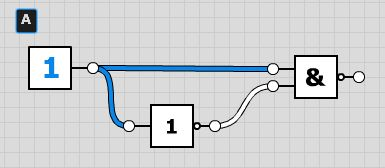
\includegraphics[width=\linewidth/2]{15}

Из-за задержки возникают ложные сигналы(помехи) в момент переключения значения А.\\
Возможность появления помехи в результате гонки сигналов называют статическим риском сбоя.\\
Для исключения таких сбоев вводят стробирование.\\
Стробирование 0 выделение из информационного сигнала части свободной от ложных сигналов.\\
Процесс стробирования переодическими сигналами называются синхронизацией, а период следования синхросигналов тактом. \\

В схемотехнике чаще всего комбинационная схема заканичвается триггером, поэтому стробирование вводят на входах триггерных схем.\\
В общем случае - вводятся в последнем каскаде.

Триггеры информационные сигналы, которых стробируются специальными переодическими сигналами навзываются синхронными триггерами.\\
Кроме исключения ложных сигналов синхронизация создает условие для одновременного изменения состояния входов триггеро,
то есть так называемая синхронная работа.


Синхронные триггеры.

Синхронные триггеры имеют один или несколько входов синхронизации. Обозначаются C. \\
Сигнал синхронизации разрешает прием сигналов с информационных входов. \\
Если вход С прямой , то при С=0 обрабатывать сигналы запрещено.\\

Синхронный RS-триггер.

$Q_{n+1} = \overline{C_n}Q_n + C_n \cdot S_n + \overline{R_n} \cdot Q_n $\\
$= Q_n \cdot (\overline{C_n} + \overline{R_n} ) + C_n \cdot S_n$\\
$ = C_n S_n + \overline{C_n R_n} \cdot Q_n$\\
$\overline{Q_{n+1}} = C_n R_n + \overline{C_n S_n} \cdot \overline{Q_n}$\\

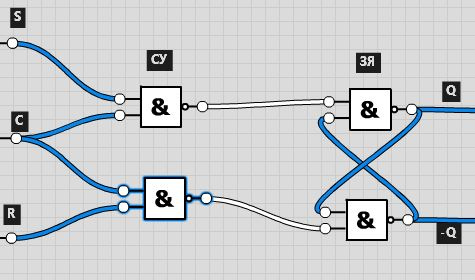
\includegraphics[width=\linewidth]{16}



$t_{u} => 3t^*_{zaderSR}$\\
$t_{p} => t_u + t_n $\\
$t_{n} => t^*_{zaderSR}$\\
$T = t_p => 4t^*_{zaderSR} $\\
$t_{max} = \frac{1}{t_p} <= \frac{1}{ 4t^*_{zaderSR}} $\\

Синхронный D-триггер.\\

$Q_{n+1} = \overline{C_n} \cdot Q_n + C_n \cdot D_n $\\
$C = 1  -> Q_{n+1} - D_n $\\


Это просто повторитель, а не запоминающая ячейка.\\
$S* = f(C_n, D_n,Q_n) $\\
$R* = p(C_n, D_n,Q_n) $\\
$S* = \overline{C_n} \overline{D_n} = \overline{C_n \cdot D_n} $\\
$R* = \overline{C_n} D_n = \overline{C_n \cdot \overline{D_n}} $\\
В данном виде требуется "лишний инвертор", надо от него избавить.\\
$R* = \overline{C_n} D_n = D_n(\overline{C_n} + \overline{C_n}) + \overline{C_n} = $\\
$D_n C_n  + D_n \overline{ C_n} + \overline{C_n} = $\\
$ D_n C_n  + \overline{C_n}(D_n + 1) = $\\
$D_n C_n + \overline{C_n}  $\\
$\overline{S^*}  + \overline{C_n}$ \\
$ \overline{S^* \cdot C_n}$\\

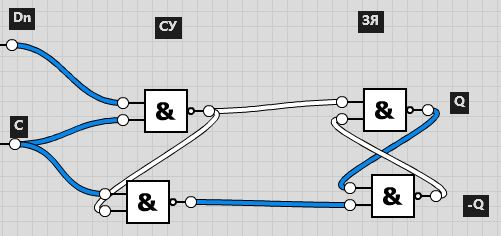
\includegraphics[width=\linewidth]{17}

DV(E) - trigger\\
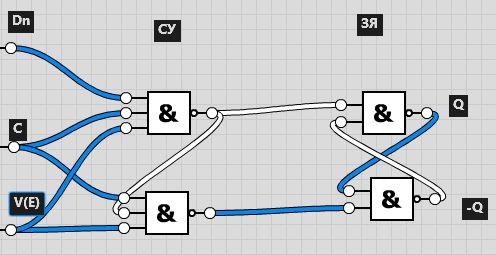
\includegraphics[width=\linewidth]{18}

Логические уравнения синхронного Д-триггера могут быть полученыил лог уравнений РС-триггера путем замены S на D, R на $\overline{D}$.\\

Асинхронный Т-триггер или счетный триггер.\\
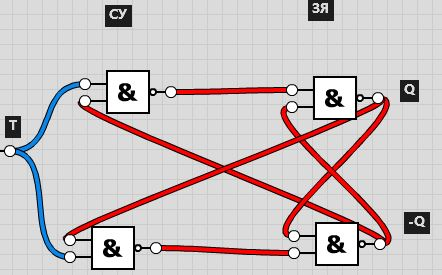
\includegraphics[width=\linewidth]{19}

По опредению он функционирует с одной таблицей перехода. \\
Триггер переключается в противоположное состояние при подаче импульса на Т.\\

$Q_{n+1} = \overline{T_n} \cdot Q_n + \overline{Q_n} + T_n = T_n +M2 Q_n $\\

$\overline{R`} = \overline{T_n} \cdot Q_n$
$\overline{S`} = \overline{T_n} \cdot Q_n$

Значения сигналов не совпадают с Д-триггером, здесь R,S не инверсные.
$t_{u} => 2t^*_{zaderSR}$\\

Если длительность входного сигнала больше длительности переходных процессов в триггере, то в сземе возникают автоколебания.
Так как при действии одного сигнала Т триггер многократно переключить в 0 и обратно.
Генерация возникает, если время импульса будет больше, чем $2t^*$.
Если же время импулься будет меньше $2t^*$, то триггер не переключиться вообще.\\
Схема работоспособна когда время импульса строго равно  $2t^*$.\\
Во-вторых никому не нужна схема, работающая на одной частоте.\\













\end{document}
